\chapter{Methods}
\section{Computational model}
The network model that was used in this research is a custom implementation
made by \textcite{sanjayImpairedDendriticInhibition2015}. This model is based
on the CA3 subfield region of the hippocampus, originally designed by~\textcite{neymotinKetamineDisruptsTheta2011}.
The model is implemented in the NEURON
simulation environment using python version 3.9.16 as an interface
\href{https://www.neuron.yale.edu}{(\url{https://www.neuron.yale.edu})}. The
model consists of 1000 neurons, which are divided into populations containing
three cell-types: 800 5-compartment pyramidal cells (three apical dendrites,
one basal dendrite, and soma), 200 1-compartment soma-inhibiting basket cells
and 200 1-compartment Oriens-Lacunosum Moleculare (O-LM) interneurons. The
original source code of the model is available on ModelDB at the following
link:
\href{http://senselab.med.yale.edu/modeldb/ShowModel.asp?model=139421}{\url{http://senselab.med.yale.edu/modeldb/ShowModel.asp?model=139421}}.

The implementation used in this research made in cooperation with Sean Gies is
part of the \textit{Neuromics} software package by Synaptica B.V. The
implementation has been modified to allow for more ease of use and to allow for
the implementation of cellular modifications and network manipulations.
Descriptions of the cell-types and their classes, network design, synaptic
connections and stimulation parameters can be found in appendix A.

The experimental source code for this research project can be found on request
on GitHub at the following link:
\href{https://github.com/SynapticaNL/Marc_network_sims}{\url{https://github.com/SynapticaNL/Marc_network_sims}}.

\begin{figure}[htbp]
    \centering
    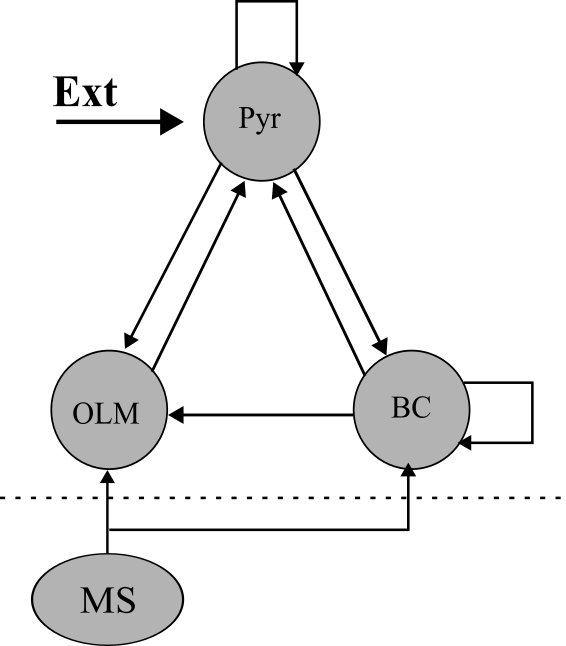
\includegraphics[width=0.7\textwidth]{model_design.png}
    \caption[Schematic of the CA3 network model]{Schematic of the CA3 network model.
        The network comprises of many microcircuits with the connectivity as shown in the above figure. Pyr cells (pyramidal), BC cells (basket cells that inhibit soma),
        O-LM cells (oriens-lacunosum moleculare interneurons that inhibit dendrites), external inputs (mainly from the entorhinal cortex) to Pyr cells, and MS (medial septum).
        BC and O-LM cells are stimulated by Pyr cells, while Pyr cells are inhibited by BC and O-LM cells.
        Recurrent connections among Pyr cells are excitatory, whereas those among BC cells are inhibitory.
        O-LM cells are inhibited by BC cells. The medial septum (MS) delivers inhibitory inputs every 150 ms to BC and O-LM cells.}\label{fig:model_design}
\end{figure}\pagebreak

\section{Model implementation: cell parameters}
The model consists of three types of neurons, each with its own set of
parameters and defined cell classes. The parameters for each cell type are
based on the following references:
\begin{enumerate}
    \item \textbf{Basket Cells}: Modeled after \textcite{wangGammaOscillationSynaptic1996},
          featuring standard dynamics for Na and K currents, along with synaptic and leak currents.
          Each cell is modeled as a single compartment and obeys the following current balance equation:
          \begin{equation}\label{eq:basket_cell}
              C_I \frac{dV_I}{dt} = I_{\text{app},I} - I_{\text{Na},I} - I_{\text{K},I} - I_{\text{L},I} - I_{\text{syn},I}
          \end{equation}

          where \(V_I\) is the membrane potential (mV), \(C_I = 1 \, \mu\text{F/cm}^2\)
          is the membrane capacitance, \(I_{\text{app},I}\) is the applied current, and
          \(I_{\text{syn},I}\) is the total synaptic current. The leak current
          \(I_{\text{L},I} = g_{\text{L},I}(V_I - E_{\text{L},I})\) has a conductance
          \(g_{\text{L},I} = 0.1 \, \text{mS/cm}^2\) and reversal potential
          \(E_{\text{L},I} = -65 \, \text{mV}\). All currents are in units of
          \(\mu\text{A/cm}^2\). The sodium \(I_{\text{Na},I}\) and potassium
          \(I_{\text{K},I}\) currents are voltage-dependent spiking currents of the
          Hodgkin-Huxley type.
    \item \textbf{O-LM Cells}: Adapted from \textcite{saragaActiveDendritesSpike2003},
          including additional currents like hyperpolarization-activated (h) and A-type currents.
          Each cell is modeled as a single compartment and obeys the following current balance equation:
          \begin{equation}\label{eq:olm_cell}
              C_O \frac{dV_O}{dt} = I_{\text{app},O} - I_{\text{Na},O} - I_{\text{K},O} - I_{\text{L},O} - I_{\text{h},O} - I_{\text{A},O} - I_{\text{syn},O}
          \end{equation}

          where \(V_O\) is the membrane potential, \(C_O = 1.3 \, \mu\text{F/cm}^2\) is
          the membrane capacitance, \(I_{\text{app},O}\) is the applied current, and
          \(I_{\text{syn},O}\) is the total synaptic current. The leak current
          \(I_{\text{L},O} = g_{\text{L},O}(V_O - E_{\text{L},O})\) with conductance
          \(g_{\text{L},O} = 0.05 \, \text{mS/cm}^2\) and reversal potential
          \(E_{\text{L},O} = -70 \, \text{mV}\). \(I_{\text{Na},O}\), \(I_{\text{K},O}\),
          \(I_{\text{h},O}\), and \(I_{\text{A},O}\) represent the transient sodium,
          delayed rectifier potassium, hyperpolarization-activated (or h) mixed-cation,
          and A-type potassium currents, respectively, all in units of
          \(\mu\text{A/cm}^2\).
    \item \textbf{Pyramidal Cells}: Based on \textcite{miglioreDendriticIhSelectivelyBlocks2004},
          incorporating compartmentalized dynamics for the complex morphology of pyramidal neurons.
          Each cell is modeled as a multi-compartmental neuron with 5 compartments: 1 for basal dendrites (Bdend),
          1 for soma, and 3 for apical dendrites (Adend1, 2 and 3). Each compartment obeys the following current balance equation:
          \begin{equation}\label{eq:pyramidal_cell}
              C_{E_k} \frac{dV_{E_k}}{dt} = I_{\text{app},E_k} - I_{\text{Na},E_k} - I_{\text{K},E_k} - I_{\text{L},E_k} - I_{\text{h},E_k} - I_{\text{A},E_k} - I_{\text{syn},E_k} + I_{\text{conn},E_k}
          \end{equation}

          where \(V_{E_k}\) is the membrane potential of compartment \(k\), \(C_{E_k}\)
          is the membrane capacitance, \(I_{\text{app},E_k}\) is the applied current,
          \(I_{\text{syn},E_k}\) is the total synaptic current, and
          \(I_{\text{conn},E_k}\) represents the current due to electrical coupling
          between compartments. \(I_{\text{L},E_k}\), \(I_{\text{Na},E_k}\),
          \(I_{\text{K},E_k}\), \(I_{\text{h},E_k}\), and \(I_{\text{A},E_k}\) denote the
          leak, transient sodium, delayed rectifier potassium,
          hyperpolarization-activated mixed-cation, and A-type potassium currents for
          compartment \(k\), respectively.
\end{enumerate}

\noindent For further elaboration of the mathematical formulation of each cell type, see appendix~\ref{ch:appendix_a}.
For the full overview of cell and compartment parameters, see appendix~\ref{ch:appendix_b}.

\section{Model implementation: synaptic connections}
The model contained three types of synaptic connections: excitatory, inhibitory
based on AMPA, NMDA and GABA-A receptors. Synapses were modeled by standard
NEURON double-exponential mechanism. This approach entailed the assignment of
specific rise \(\tau_1\) and decay \(\tau_2\) time constants, which correspond
to the temporal profiles of conductance increase and subsequent decline,
respectively, following a synaptic event. The conductance values, indicative of
synaptic efficacy, were varied according to the type of presynaptic and
postsynaptic neuron pairing, as well as the subtype of receptor involved (AMPA,
NMDA, or GABA-A). These parameters informed the simulation of synaptic inputs,
which govern the depolarization and hyperpolarization events in the
postsynaptic neuron membrane, thereby influencing the temporal patterns of
neuronal firing and network activity. These parameters adhere to the following formula:

\begin{equation}\label{eq:synaptic_conductance}
    g(t) = \frac{g_{\text{max}}}{\tau_2 - \tau_1} \left( e^{-\frac{t}{\tau_2}} - e^{-\frac{t}{\tau_1}} \right)
\end{equation}

The synaptic conductance at a given time \(t\) after a presynaptic spike is represented by \(g(t)\), where \(g_{\text{max}}\) indicates the peak conductance measured in NanoSiemens (nS).
The rise and decay of the synaptic conductance are characterized by the time constants \(\tau_1\) and \(\tau_2\), respectively, both of which are measured in milliseconds (ms).
Here, \(t\) stands for the time elapsed following the arrival of the presynaptic spike.
This model effectively describes the dynamic behavior of synaptic conductance, which initially rises during the onset phase and subsequently undergoes a more prolonged decrease, a pattern common to both excitatory and inhibitory postsynaptic potentials (EPSPs and IPSPs).
The variation in the time constants \(\tau_1\) and \(\tau_2\) facilitates the adjustment of the synaptic response's time profile, with \(\tau_1\) influencing the speed of onset and \(\tau_2\) affecting the length of the conductance alteration.
For the parameters used, see Table~\ref{table:compartment_dependent_parameters} and~\ref{tab:synaptic_parameters}.
\begin{table}[htbp]
    \centering
    \caption[Compartment dependent parameters]{Compartment dependent parameters used in the formulations of the three neuronal cell types according to equation~\ref{eq:synaptic_conductance}.
        See appendix~\ref{ch:appendix_a} for the full equations.
        The ionic conductances are in mS/cm\(^2\).}\label{table:compartment_dependent_parameters}
    \begin{tabular}{l|cccccccccc}
        \hline
        \hline
               & \( g_{h} \) & \( g_{A} \) & \( g_{Na} \) & \( g_{K} \) & \( V_{50} \) & \( b \) & \( c \) & \( d \) & \( e \) & \( f \) \\
        \hline
        Bdend  & 0.1         & 48          & 32           & 10          & -82          & 1       & 4       & 1.5     & 11      & 0.825   \\
        Soma   & 0.1         & 48          & 32           & 10          & -82          & 0.8     & 4       & 1.5     & 11      & 0.825   \\
        Adend1 & 0.2         & 72          & 32           & 10          & -82          & 0.5     & 4       & 1.5     & 11      & 0.825   \\
        Adend2 & 0.4         & 120         & 32           & 10          & -90          & 0.5     & 2       & 1.8     & -1      & 0.7     \\
        Adend3 & 0.7         & 200         & 32           & 10          & -90          & 0.5     & 2       & 1.8     & -1      & 0.7     \\
        \hline
        \hline
    \end{tabular}
\end{table}
\pagebreak

\noindent
The synaptic connections between neurons were implemented
as follows:

\begin{table}[htbp]
    \centering
    \caption[Synaptic Parameters for the Connectivity Between Neurons in the Model]{Synaptic Parameters for the Connectivity Between Neurons in the Model: Pre- and postsynaptic receptor types are given for each cell type.
        The time constants \(\tau_1\) and \(\tau_2\) are in milliseconds.
        \(\tau_1\) is the rise time constant, the time it takes for synaptic conductance to increase from baseline to peak.
        \(\tau_2\) is the decay time constant, the time it takes for the conductance to decrease from peak to baseline.
        The conductance indicates the strength of the synaptic connection and its ability to conduct ionic current across the postsynaptic membrane.
        This influences the extent to which the synaptic input can depolarize the postsynaptic neuron and is in nanoSiemens (nS).}\label{tab:synaptic_parameters}
    \begin{tabular}{lllccc}
        \hline
        Presynaptic & Postsynaptic & Receptor & \(\tau_1\) (ms) & \(\tau_2\) (ms) & Conductance (nS) \\
        \hline
        Pyramidal   & Pyramidal    & AMPA     & 0.05            & 5.3             & 0.02             \\
        Pyramidal   & Pyramidal    & NMDA     & 15              & 150             & 0.004            \\
        Pyramidal   & Basket       & AMPA     & 0.05            & 5.3             & 0.36             \\
        Pyramidal   & Basket       & NMDA     & 15              & 150             & 1.38             \\
        Pyramidal   & OLM          & AMPA     & 0.05            & 5.3             & 0.36             \\
        Pyramidal   & OLM          & NMDA     & 15              & 150             & 0.72             \\
        Basket      & Pyramidal    & GABA-A   & 0.07            & 9.1             & 0.72             \\
        Basket      & Basket       & GABA-A   & 0.07            & 9.1             & 4.5              \\
        Basket      & OLM          & GABA-A   & 0.07            & 9.1             & 0.0288           \\
        OLM         & Pyramidal    & GABA-A   & 0.2             & 20              & 72               \\
        MS          & Basket       & GABA-A   & 20              & 40              & 1.6              \\
        MS          & OLM          & GABA-A   & 20              & 40              & 1.6              \\
        \hline
    \end{tabular}
\end{table}

\noindent For the full overview of synaptic parameters, see appendix~\ref{ch:appendix_b}.
\pagebreak

\section{Model implementation: stimulation and noise}
The model was activated by external inputs originating from the entorhinal
cortex, which were then transmitted to the pyramidal cells. Background random
excitatory and inhibitory inputs were received by the O-LM, basket cells, and
the soma of the pyramidal cells via their AMPA, NMDA, and GABA-A receptors as
shown in Table~\ref{tab:synaptic_parameters}. The mechanism by which noise was
applied to the model was defined via NEURON simulator's \textit{NetStim}
object. This object type generated spike train according to a set of parameters
such as stimulus interval, noise variability (Poisson-like), weight, target,
start and delay times. These parameters can be viewed in Appendix A.

Similarly, the distal dendritic compartments of the pyramidal cells also
received comparable inputs through the same types of receptors. Connections
such as O-LM to pyramidal cell, basket to pyramidal cell, basket-basket
recurrent connections, and medial septum to O-LM and basket cell connections
were mediated through GABA-A receptors. Additionally, the medial septum
provided inhibitory inputs to the basket and O-LM cells at intervals of 150 ms.

\section{Simulations}
For the simulations, the model was implemented in NEURON version 7.6.3. The
simulations were run on a Linux GNOME (v22.04) desktop computer with 2 Xeon CPU
E5--2699 v3 CPUs with 32 physical cores @ 2.3GHz for multi-threading, a Nvidia
GTX 4060 graphics card, and 256 GB of RAM\@. Trials were run for 5000 ms with a
time integration step of 0.1 ms resulting in 50.000 simulation steps per trial
dataset. Random seeds were used to generate the external noise, connections and
cells for each trial and remained constant between trials and between
experiments. The number of trials varies between experiments and are specified
in their respective sub-sections that follow. In the network, the individual
cells were assigned a global identifier (GID) to which all the data was
associated in the same ascending order for each trial. The first 800 cells were
always pyramidal cells, the next 200 were basket cells and the last 200 were
O-LM cells. For each trial, the individual cell spike times were saved for the
entire duration of the simulation. Pyramidal cell membrane soma voltage data
was saved per cell in order to calculate the LFP signal (necessary for
theta-gamma calculations). In all simulations the LFP is calculated by
taking the sum of the differences in membrane potential of the distal apical
and basal dendritic compartments of all cells in the pyramidal population.

\subsection{Baseline activity}
In order to obtain baseline activity in the network as shown in Figure
~\ref{fig:model_design}, current injections were added (\textbf{Pyramidal
    cells:} 50 pA\@; \textbf{O-LM cells:} -25 pA). At Baseline, the network
generates theta-modulated gamma oscillations activity. This activity was
measured from the Local Field potential (LFP) in the network. The LFP was
simulated by a sum difference between membrane potential of the distal apical
and basal dendritic compartment over all pyramidal cells. As discussed in the
cell parameters section, all cells contained leak current, transient sodium
current \(I_{\text{Na}}\), and delayed rectifier current \(I_{K, \text{-}
        \text{dr}}\) to allow for action potential generation. On average, the firing
rates were \(2.36 \pm 0.024\) Hz for pyramidal cells, \(16.05 \pm 0.15\) Hz for
basket cells and \(0.96 \pm 0.027\) Hz for O-LM interneurons at baseline in the
original \parencite{sanjayImpairedDendriticInhibition2015}. However, it should
be noted that our custom implementation of the same model had a slightly
lowered baseline (see the results section). The reason for this discrepancy is
unknown and is a potential source of error in the results. 50 trials total were
done for the baseline activity and averaged.

\subsection{Model validation}
In order to test the implementation of the model, results from the article were
replicated, namely Figures 6A, B and C from
\textcite{sanjayImpairedDendriticInhibition2015}. In this replicated experiment
the O-LM to pyramidal cells connection weight was reduced in decrements of 0.1x
times the baseline from 1.0 to 0.0. In addition to reduced connection strength,
the external noise fed into the pyramidal cells was increased in increments of
0.1X times the baseline from 1.0 to 2.0. By reducing the connectivity from O-LM
to pyramidal cells, dendritic inhibition was impaired and potential
epileptiform activity was induced.

The original results on which the validation experiment focussed on, were the
following three aspects: changes in firing rates per population, the changes in
dominant theta and gamma frequencies, and finally the changes in the power of
the theta and gamma oscillations (see
Figure:~\ref{fig:validation_original_results}). The numerical results from are
in the following table:

\begin{table}[htbp]
    \centering
    \caption[Summary of Original Network Simulation Parameters and Results]{Overview of Original Network Simulation Settings and Outcomes.
        This table contains all the original results of Figure 6 from the \textcite{sanjayImpairedDendriticInhibition2015} article.
        Variations in the firing rates of single cells, alongside theta and gamma oscillations within the local field potential, as well as the alterations in their intensity upon the decrease of dendritic inhibition and the concurrent enhancement of external stimuli to the pyramidal neurons.}\label{tab:original_validation_results}
    \begin{adjustbox}{width=\textwidth}
        \begin{tabular}{ccccccccc}
            \hline
            OLM-Pyr Wt & External Wt & \CellWithForcedBreak{Pyr (Hz)                                                          \\ + Std} & \CellWithForcedBreak{BWB (Hz) \\ + Std} & \CellWithForcedBreak{OLM (Hz) \\ + Std} & \CellWithForcedBreak{Theta \\ Freq (Hz)} & \CellWithForcedBreak{Theta power \\ (mV\textsuperscript{2} Hz\textsuperscript{-1})} & \CellWithForcedBreak{Gamma \\ Freq (Hz)} & \CellWithForcedBreak{Gamma power \\ (mV\textsuperscript{2} Hz\textsuperscript{-1})} \\
            \hline
            1x         & 1x          & 2.36 ± 0.024                  & 16.05 ± 0.15 & 0.96 ± 0.027 & 6.7 & 5.35 & 33.2 & 2.55 \\
            0.8x       & 1.2x        & 2.66 ± 0.029                  & 19.88 ± 0.11 & 1.11 ± 0.03  & 6.7 & 5.4  & 32.5 & 2.4  \\
            0.6x       & 1.4x        & 2.9 ± 0.03                    & 21.04 ± 0.15 & 1.42 ± 0.03  & 6.7 & 4.1  & 32.4 & 5.3  \\
            0.4x       & 1.6x        & 3.19 ± 0.033                  & 22.15 ± 0.15 & 1.93 ± 0.03  & 6.7 & 2.2  & 31.7 & 3.6  \\
            0.2x       & 1.8x        & 3.67 ± 0.036                  & 23.97 ± 0.15 & 2.64 ± 0.036 & 6.7 & 2    & 32.7 & 6.5  \\
            0.1x       & 1.9x        & 4.24 ± 0.038                  & 26.98 ± 0.15 & 3.35 ± 0.034 & 6.7 & 1.16 & 33.9 & 11.4 \\
            0.05x      & 1.95x       & 4.5 ± 0.04                    & 21.68 ± 0.25 & 3.69 ± 0.033 & 6.7 & 0.65 & 37.8 & 1.55 \\
            0x         & 2x          & 6.14 ± 0.054                  & 24.26 ± 0.44 & 4.98 ± 0.035 & 0   & 0    & 38.8 & 1.32 \\
            \hline
        \end{tabular}
    \end{adjustbox}
\end{table}

\begin{figure}[htbp]
    \centering
    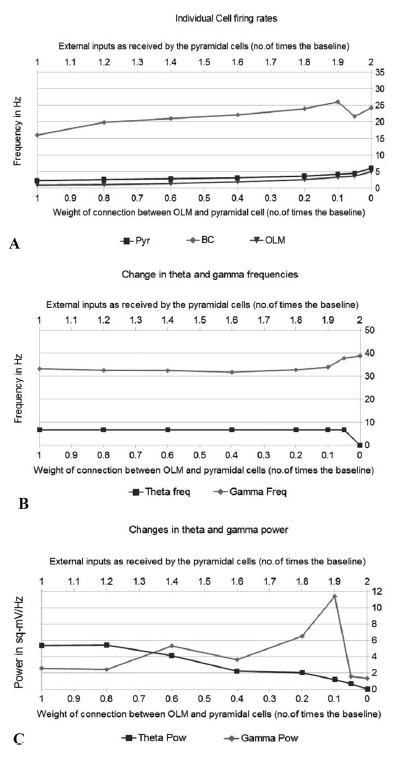
\includegraphics[width=0.65\textwidth]{model_validation_original_results.png}
    \caption[\textcite{sanjayImpairedDendriticInhibition2015} article results]{\textcite{sanjayImpairedDendriticInhibition2015} article results: Figure 6.
        A validation experiment was conducted to replicate the results of scenario 2 from the original article.
        This was done in order to verify the implementation of the model. The experiment involved reducing the
        connection strength from O-LM to pyramidal cells and increasing the
        external noise fed into the pyramidal cells. The firing rates per population (A), dominant frequencies in the theta-gamma bands (B) and their respective average power (C) was investigated.
        The results were compared to the original article to verify the implementation of the model (see Results section).}\label{fig:validation_original_results}
\end{figure}

\subsection{Sodium and potassium variants}
In this experiment, the sodium and potassium conductances of the all cell types
cells were changed from 0.5x to 1.5x times the baseline in increments of 0.1.
The changes were induced in separate experiments for each of the three cell
types, so 6 experiments in total were conducted: 3 for sodium and 3 for
potassium. These induced changes were done in order to investigate the effect
of the conductances on the network activity and the influence of individual
cell types on the same metrics as in the model validation experiment. 20 trials
each were done per condition (6 total conditions) and the results were
averaged.

\subsubsection{Visualization of Neuronal Activity Variants}
This section outlines the analytical approach adopted for visualizing the
neuronal activity within our network model under different experimental
conditions. Specifically, we focused on plotting the firing rates, theta-gamma
frequencies, and theta-gamma power across all neuronal populations (pyramidal,
basket, and O-LM cells) for variants induced by alterations in sodium and
potassium conductance levels.

\subsubsection{Firing Rate Analysis}
We initiated our analysis by examining the firing rates across different cell
populations. A comparative visualization was generated to juxtapose the mean
firing rates under sodium and potassium variant conditions, utilizing a grid
layout for a side-by-side comparison. Each plot incorporated error bars to
represent the standard error of the mean (SEM), thereby conveying the
variability inherent in our simulation trials. Cell populations were
differentiated by distinct markers and colors to facilitate clear distinction
between pyramidal, basket, and O-LM cells across varying conditions.

\subsubsection{Theta-Gamma Frequency Analysis}
Subsequent to firing rate analysis, we delved into the investigation of theta
and gamma frequency bands. For each variant type (sodium and potassium), theta
and gamma frequencies were plotted on a \(2\times2\) grid, delineating the mean
frequency values extracted from the simulation data. This approach allowed for
an intuitive understanding of the oscillatory dynamics prevalent in the network
under different ionic conductance conditions, highlighting potential shifts in
theta-gamma coupling associated with epileptiform activities.

\subsubsection{Theta-Gamma Power Analysis}
In addition to the frequency analysis, the power of theta and gamma oscillations were quantified.
This step aimed to investigate the intensity of oscillatory activity within these critical frequency bands.
Similar to our frequency analysis, a \(2\times2\) grid layout facilitated the comparison of theta and gamma power
across sodium and potassium variants. This visual representation served to
elucidate variations in oscillatory power, potentially correlating with changes
in network excitability and synchronization under altered ionic conditions.

\subsubsection{Power Spectral Density (PSD) Calculation}
The aforementioned theta-gamma analyses used the \lstinline{calc_psd} function to compute the power spectral density (PSD) of an LFP signal, focusing on theta (3--12 Hz) and gamma (30--80 Hz) frequencies.
Initial signal processing includes discarding the first millisecond to avoid transient effects and down-sampling according to a predefined maximum frequency (\textit{fmax}).
The PSD calculation uses a Fast Fourier Transform (FFT) approach, adjusting for the signal mean.
For both theta and gamma ranges, the function identifies relevant frequencies, calculates mean power by averaging power values within these ranges, and identifies the dominant frequency by locating the frequency with the maximum power value.
This analysis facilitated the quantification of signal power and rhythmic activity within specific frequency bands, essential for understanding neural dynamics in these ranges.

\subsection{External noise variants}
In this experiment, the external noise fed into the distal dendrites of
pyramidal cells was set a new baseline for the 1.0x condition, which was 20 times that of the original
\textcite{sanjayImpairedDendriticInhibition2015} model. Excitatory inputs were fed through
AMPA and NMDA receptors. Reduced O-LM to pyr connections were kept at 10\% of
the original baseline. This was done because in the original article, epileptic activity was induced by feeding in 20 times
more external noise at reduced dendritic inhibition.

This condition was tested as a special condition in Figure 7 of the article,
and was expanded upon because of the occurrence of a depolarization block in
the basket cell spike activity. This depolarization block occurrence was
assumed to be the epileptic state in which the network is found at such
conditions. This new baseline was changed times a range of pyramidal noise
factors of the following values: 0.65, 0.70, 0.75, 0.80, 0.85, 0.90, 0.95,
1.00, 1.10, 1.20, and 1.30. In addition to the range of noise factors,
pyramidal conductances \(g_{\text{Na}}\) and \(g_{\text{K}}\) were modified
over a range of 0.5x to 1.5x times the baseline in increments of 0.1. 15 trials
were done per noise condition and the results were averaged.

\subsubsection{Detection of epileptiform activity (Experiments: External Noise and Recurrent Connection strength variants)}
The detection of epileptic activity depends on the spiking activity of the
basket cells, which according to results of Figure 7 from the
\textcite{sanjayImpairedDendriticInhibition2015} article occurs in the presence
of great external drive from the pyramidal cells of at least 20 times the
baseline and with reduced dendritic inhibition by the O-LM cells. Detection of a
depolarization block in the basket cells was done by calculating the convoluted
fire rates of the basket cell population.


\noindent The systematic approach to analyzing basket cell firing rates through convolution with a Gaussian window was as follows:
\begin{itemize}
    \item \textbf{Extracting Spike Times:} The \lstinline{get_spike_times_for_basket_cells}
          function is used for iterating over a range of GIDs. This process collects spike times from
          all basket cells and concatenates them, constructing a continuous signal of neural activity.

    \item \textbf{Creating Time Series:} Spike times are converted into a binary series
          using \lstinline{create_time_series}. Each neural firing event is denoted by a '1' in a
          zero-initialized array at the corresponding time index.

    \item \textbf{Applying Gaussian Convolution:} The \lstinline{apply_gaussian_convolution}\newline
          function smooths the time series. It convolves the series with a Gaussian window, normalized
          to sum to one, yielding a signal that mirrors the firing rates over time.

    \item \textbf{Summing Convolved Signals:} Collective firing behavior is analyzed by
          \lstinline{get_convolved_signal_per_neuron}. It applies Gaussian convolution to individual
          neuron time series and sums them, forming an aggregated firing rate signal.

    \item \textbf{Detecting Depolarization Blocks:} The \lstinline{detect_depolarization_blocks}
          function identifies reduced activity periods by analyzing the convolved signal for intervals
          that remain below a set threshold for a specified minimum duration.
\end{itemize}

\noindent
This method for detecting depolarization blocks in the basket cell population
and convolution of spike activities was also used for the recurrent
connection strength variants experiment below. See the example in Figure~\ref{fig:depolarization_block_basket_cells}.

\begin{figure}[htbp]
    \centering
    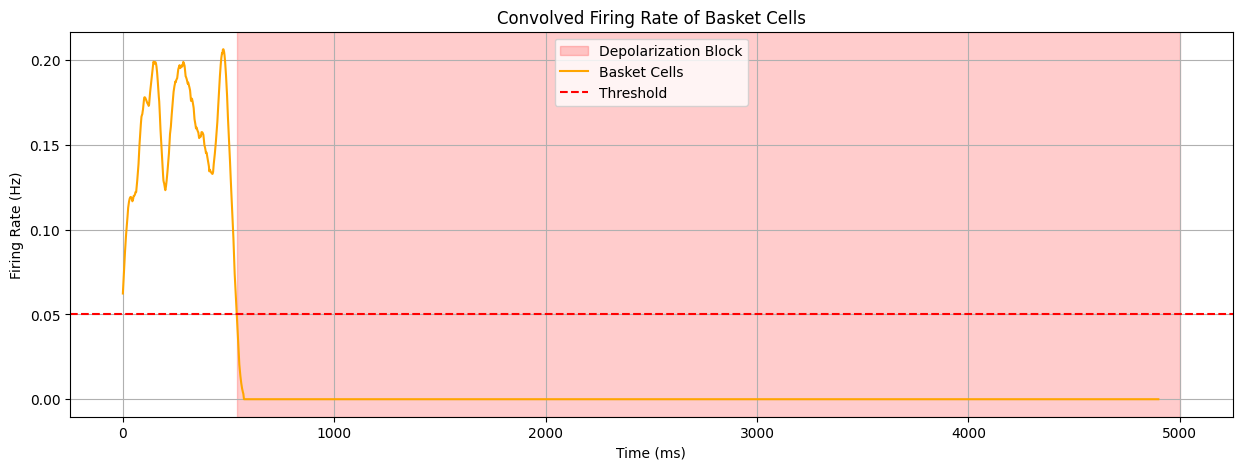
\includegraphics[width=1.0\textwidth]{Depolarization_block_basket_cells.png}
    \caption[Depolarization block in basket cells]{Depolarization block in basket cells. Example of a single trial where a depolarization block is found in the convoluted spike activity signal as a flat-line at 0 Hz. The firing rate is in Hz (y-axis) and the signal is calculated over the entire duration of the trial (5000 ms).
        Note that the signal has to pass the threshold for an extended period of 100 ms to be considered a DPB\@.
        In addition, the first 50 ms are excluded from detection to avoid false positives. This detection method was done for each individual trial.}\label{fig:depolarization_block_basket_cells}
\end{figure}
\pagebreak

\subsubsection{Analysis of External Noise Variants}
This section elaborates on the methodological approach undertaken to assess the
impact of varying levels of external noise on pyramidal cells, with the aim of
understanding its influence on depolarization block occurrences within the
network. The experiment's premise was based on the hypothesis that adjusting
the external noise could modulate the epileptic state, characterized by
depolarization blocks, within the neural network.\\

\noindent The analysis was structured as follows:
\begin{enumerate}
    \item \textbf{Event Detection and Quantification:} For each variant of external noise levels, depolarization events were systematically identified. These results were quantified per trial. This process involved the enumeration of depolarization events, accumulation of their start and end times, and the computation of the overall duration of these events within each trial.

    \item \textbf{Statistical Analysis:} Subsequent to the detection of depolarization events, the analysis proceeded with the calculation of average event duration and the computation of the percentage of trials exhibiting depolarization blocks. Furthermore, the mean delay and standard deviation for the onset of depolarization events were determined to gauge the temporal dynamics of the network's response to varying noise levels.

    \item \textbf{Data Visualization:} To concisely present the findings, the analysis results were visualized through matrix plots. These plots delineated the relationship between pyramidal conductances (\(g_{\text{Na}}\) and \(g_{\text{K}}\)) and the observed network behavior under different external noise conditions. The visualizations highlighted the proportion of trials with depolarization blocks and detailed the temporal onset characteristics of these events, facilitating an intuitive understanding of the network's epileptic susceptibility.
\end{enumerate}

\noindent The investigative focus on external noise variants sought to delineate
the conditions under which the network transitions into an epileptic state, as indicated by the
presence of depolarization blocks and the average delay in the onset of a DPB (including STD).
\pagebreak
\subsection{External noise: Burst analysis}
Further analysis was conducted to investigate the burst dynamics of pyramidal
and basket cell activity based on the observations done in the initial
increased noise experiment. This experiment involved looking at the temporal
shift in detected bursts surrounding the onset of a depolarization block event
in the basket cell population.

\subsubsection{Detection of Epileptiform Activity and Burst Analysis}
This experiment employed leveraging convolved spike activities and burst detection within
neural populations to detect epileptiform activity. The approach was predicated on analyzing the temporal
dynamics of neuronal firing rates, specifically focusing on the basket and
pyramidal cell populations. A critical aspect of this analysis was the
identification and analysis of bursts in relation to the onset of
depolarization blocks (DPBs), including the possible variance in burst intensity.\\

\noindent The unified methodology proceeded as follows:
\begin{itemize}
    \item \textbf{Identification of Depolarization Block Onset:} A custom python function \lstinline{find_depolarization_block} was employed to scan the simulation data for periods devoid of spiking activity within a specified window across basket cell populations.
          This step was crucial in pinpointing the initial point of a depolarization block, thus serving as a reference for the subsequent analysis.

    \item \textbf{Preparation and Convolution of Spike Activities:} Spike times were aggregated and subjected to a Gaussian filter, smoothing the data to represent neural firing rates over time effectively.
          This step facilitated the identification of significant patterns in relation to the DPB onset.

    \item \textbf{Burst Detection and Temporal Analysis:} The convolved spike activities were analyzed using a burst detection algorithm, identifying significant increases in activity as bursts.
          These were classified based on their occurrence relative to the DPB onset—focusing on the last burst before, the second-last burst before, and the first burst after the onset. This classification shed light on the changes in neural dynamics preceding and following a depolarization block.

    \item \textbf{Analytical Assessment and Summarization of Findings:} Start and end times were determined for detected bursts, as well as peak activity levels.
          This comprehensive analysis of convolved spike activities and burst dynamics provided a detailed view of the neural mechanisms during critical phases of epileptiform activity.
\end{itemize}

\noindent The experiment utilized a 100 ms window and a 0.1 ms time step throughout the 5000 ms simulation duration, resulting in 50,000 indices for spike detection.
The absence of basket cell firing within this window indicated a DPB, which was critical for burst detection.
This methodology offered a nuanced understanding of epileptiform dynamics, highlighting the transitions of neural populations into and out of depolarization blocks which are indicative of epileptic activity in the network.
Note that in the burst analysis the 1D-Gaussian convolution was performed on a histogram of the spike times of cells. Whereas in the previous convolution for the matrices, the convolutions were performed using a binary time series of the spike times.

\begin{figure}[htbp]
    \centering
    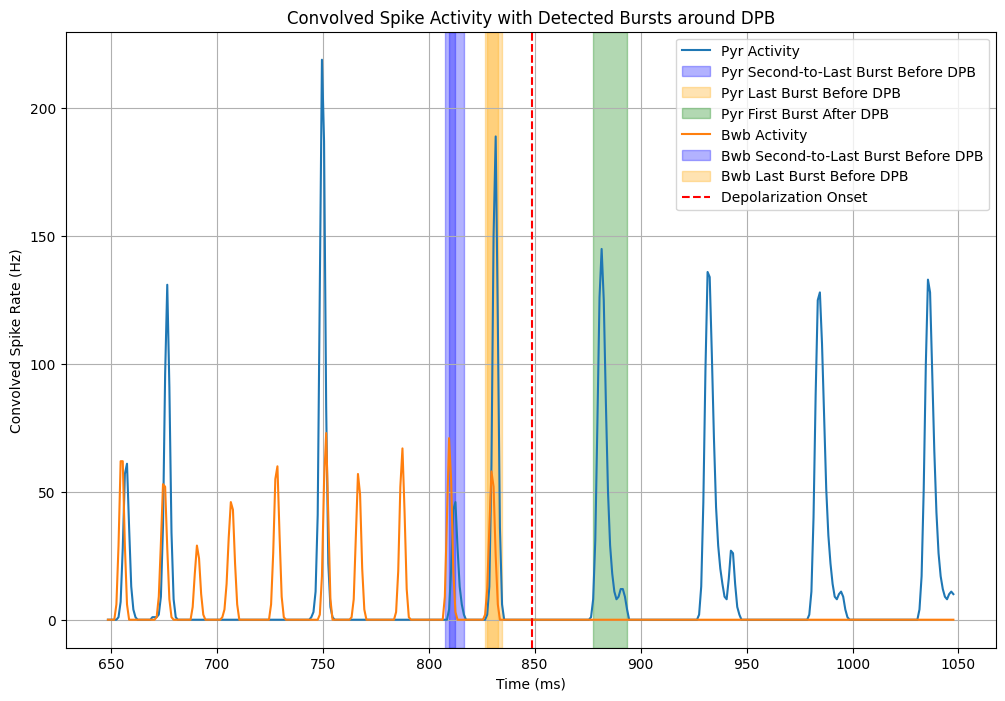
\includegraphics[width=1.0\textwidth]{Convolved_Burst_detection_DPB_example.png}
    \caption[Burst detection example]{Burst detection example. Example of a single trial where bursts in the neural populations are detected near the onset of a DPB using convoluted spike activity signals. The firing rate is in Hz (y-axis) and the signal is calculated over the entire duration of the trial (5000 ms).
        The onset of a depolarization block in basket cells is indicated by a red dashed vertical line. The last and second to last bursts before, and the first burst after the DPB were detected and used for analysis.
        Note that the signal has to pass the threshold for an extended period of 100 ms to be considered a DPB\@.
        In addition, the first 50 ms are excluded from detection to avoid false positives. This detection method was done for each individual trial.}\label{fig:example_burst_detection}
\end{figure}
\pagebreak

\subsection{Recurrent connection strength variants}
This section describes the methodology employed to analyze the effects of
varying recurrent connection strengths between basket cells on the incidence
and characteristics of depolarization blocks within the network. This analysis
aimed to explore the potential of modulating soma inhibition strength to
mitigate epileptic activity and restore baseline network dynamics.

The experiment adjusted the recurrent connection strength across a range of
multipliers (1.00, 1.05, 1.10, 1.15, and 1.20 times the baseline), concurrently
with modifications to \(g_{\text{Na}}\) and \(g_{\text{K}}\) within a plus or
minus 25\% range of the baseline. The connection weight from O-LM cells to
pyramidal cells was fixed at 10\%, facilitating the induction of depolarization
blocks under a 20x external noise condition on pyramidal cells. A total of 15
trials were conducted for each condition, and the results were averaged for
analysis.

\subsubsection{Analysis of Recurrent Connection Strength Variants}
\noindent The analysis procedure was as follows:
\begin{enumerate}
    \item \textbf{Event Detection and Aggregation:} The analysis began by identifying depolarization events across trials for each variant of the recurrent connection strength. This involved counting the number of depolarization events, their start and end times, and the total duration of depolarization within each trial. Trials devoid of depolarization events were separately tallied.

    \item \textbf{Statistical Computation:} For trials exhibiting depolarization events, the average duration of these events was calculated. Additionally, the percentage of trials manifesting depolarization events and the statistical measures (mean and standard deviation) concerning the onset times of these events were determined.

    \item \textbf{Matrix Visualization:} The analyzed data were visualized using matrix plots to illustrate the relationship between the recurrent connection strength variants and the properties of depolarization events under different \(g_{\text{Na}}\) and \(g_{\text{K}}\) conditions. These plots highlighted the percentage of trials with depolarization blocks and the count of depolarization events, offering insights into the efficacy of soma inhibition strength adjustments in modulating epileptic activity.
\end{enumerate}

\noindent
This analytical approach facilitated a comprehensive examination of the impact of modifying recurrent connection strengths among basket cells on the network's susceptibility to epileptic disruptions.
Through statistical and visual analyses, the dynamics governing epileptiform activity and the potential for intervention was investigated through targeted manipulation of inhibition mechanisms within the neural circuitry.
\pagebreak

\noindent For detecting depolarization blocks in the basket cell population, the
methodology was as follows:
\begin{itemize}
    \item Establishing a signal threshold indicating a depolarization block.
    \item Excluding initial transient analysis to prevent false positives.
    \item Identifying threshold crossings that mark the start and end of depolarization
          blocks.
    \item Applying a minimum duration filter to these blocks.
    \item Summarizing and reporting the total duration of all valid depolarization blocks
          in the trial.
\end{itemize}

\noindent A check was performed if the convoluted signal remained beneath a fixed
threshold of 0.001 for at least 100 ms. This threshold was defined non-zero,
yet tiny as in the depolarization block there are no firing neurons in the
basket population. The first 50 ms of the signal were excluded to avoid false
positives. If the signal remained beneath the threshold for at least 100 ms,
the condition was considered to be in a depolarization block state. This was
done for each trial individually. An example of this can be seen in Figure~\ref{fig:depolarization_block_basket_cells}.

